\chapter{Anomaly Detection}
\label{cha:anomaly_detection}
\epigraph{
  The field of anomaly detection is very broad and many different fields have
  developed a great variation of different methods for finding outliers.  This
  work is focusing on detecting anomalies in sequences by predicting the
  expected evolution of a time series and comparing this prediction to real
  observations (or simply: the truth).  Before describing this process in more
  detail, this chapter defines the different kinds of anomalies that exist in
  sequences and briefly summarizes two other, common detection methods
  for sequence outlier detection.
}

\section{Anomalies}
\label{sec:anomalies}
An anomaly (or outlier) refers to a pattern in a dataset that does not match
an expected behaviour.
In time series, there are two basic types of anomalies:
\begin{enumerate}

  \item \emph{Simple anomalies}, describe instances that can be considered as
    an outlier only with respect to their value. This is the most basic kind of
    anomaly which can easily be caught by ordinary, statistical, range-based
    detection algorithms. The anomaly in Fig.~\ref{fig:intro_point_anomaly}
    consists of a single instance and is hence called a \emph{point} anomaly.
    \begin{figure}
      \centering
      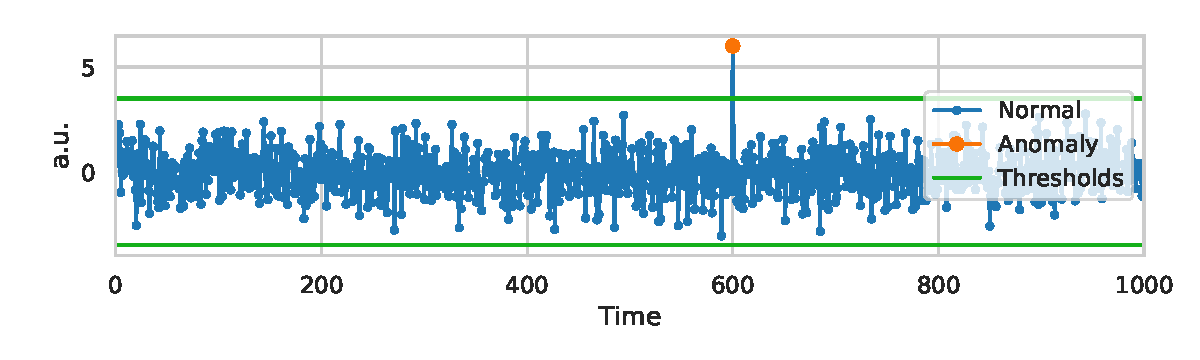
\includegraphics[width=\linewidth]{intro_point_anomaly.pdf}
      \caption{The simple point anomaly can easily be detected by appropriate
      thresholds (green lines).}
      \label{fig:intro_point_anomaly}
    \end{figure}

  \item \emph{Contextual anomalies} are patterns that are only anomalous within
    a certain context, but not otherwise. In time series, the context is
    provided by two attributes: The \emph{contextual attribute} is typically
    time itself, while the \emph{behavioural attributes} describe the actual
    values of the examined dataset. Fig.~\ref{fig:intro_context_anomaly} shows
    a contextual anomaly consisting of several abnormal points, which is
    referred to as a \emph{discord} or \emph{subsequence} anomaly.
    \begin{figure}
      \centering
      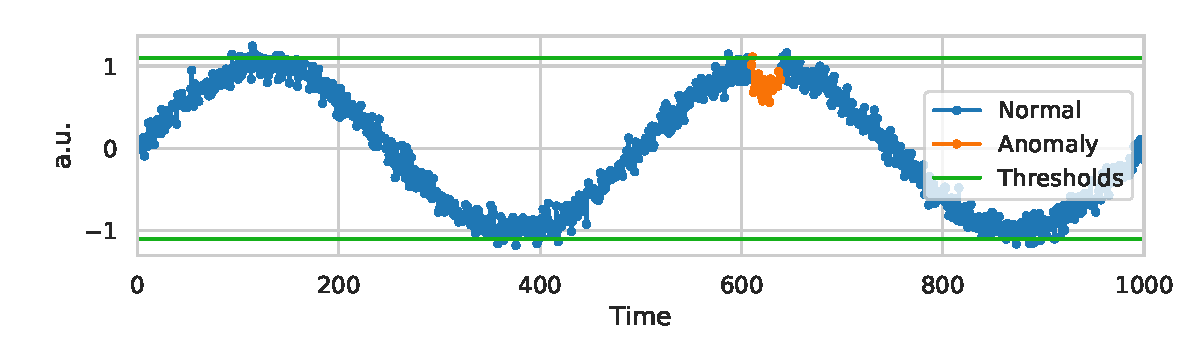
\includegraphics[width=\linewidth]{intro_context_anomaly.pdf}
      \caption{Contextual anomalies are not detectable with simple statistical
      methods without causing a large number of false positives.}
      \label{fig:intro_context_anomaly}
    \end{figure}
\end{enumerate}


\newpage
\section{Techniques}
\label{sec:techniques}

The difficulty of anomaly detection stems from the fact that the patterns that
are searched for are typically not known.  Different fields have come up with a
large number of different approaches for the detection of the different kinds
of anomalies. Two such approaches  are sketched below: \emph{proximity-based}
techniques, and {\em information theoretical} approaches [\cite{AggarwalCharuC2017}].

\subsection{Proximity-based Anomaly Detection}
\label{sub:proximity_based_anomaly_detection}

By applying certain transformations to segments of a time series, a segment can be
mapped into a multidimensional vector space. The proximity can then be
calculated for example with the Euclidean distance, which opens up the whole
range of proximity-based outlier detection methods, such as cluster, distance,
and density based techniques.

The trivial example of such a transformation is to just consider segments of
length $n$ as a vector of length $n$.  Other approaches include \emph{Discrete
Fourier Transforms} (DFT) or \emph{Discrete Wavelet Transforms} (DWT), the
simplest of which is the \emph{Haar Wavelet}. A Haar Wavelet decomposition is
sketched in Fig.~\ref{fig:haar_wavelets}, a more detailed description of how
wavelet transformations work is given in [\cite{AggarwalCharuC2017}]. The
advantage of transforming a sequence into a vector of wavelet coefficients is
that the coefficients directly represent short-term and long-term dependencies.
This enables a reduction of the dimensionality of the space that has to be
analyzed depending on the nature of the problem. For example, frequencies above
a certain threshold can be ignored.  The application of proximity-based methods
naturally becomes much more effective on the transformed sequences. Depending
on the nature of the dataset different transformations are more effective.  For
sequences with dominant periodic parts the DFT works better, while series with
discontinuities are well represented by the Haar-DWT.

\begin{figure}
  \centering
  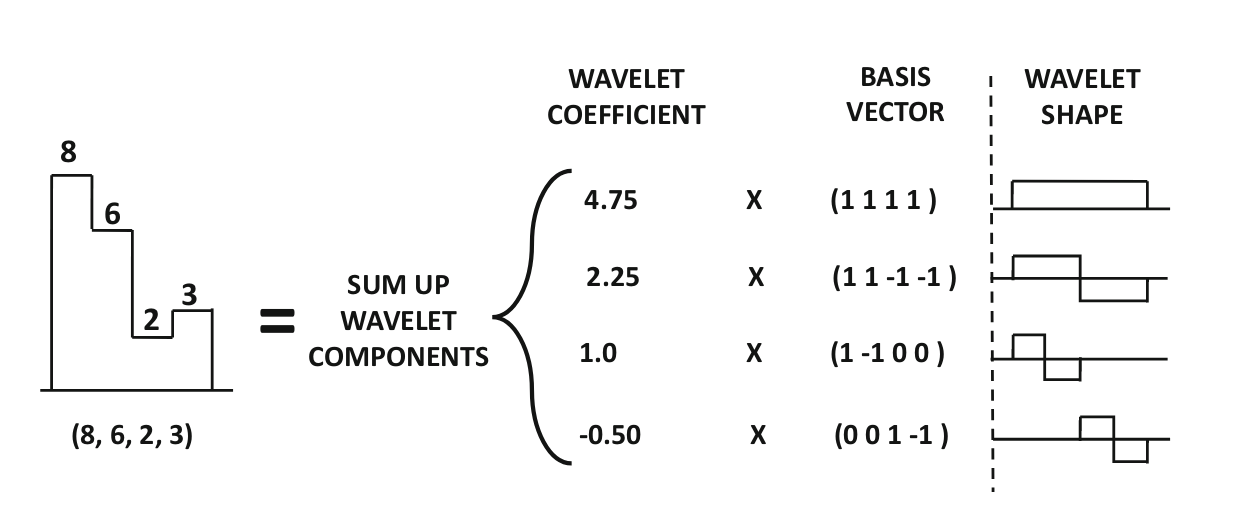
\includegraphics[width=0.9\linewidth]{haar_wavelets.png}
  \caption{Haar wavelet decomposition of series of length 4
  [\cite{AggarwalCharuC2017}.}]
  \label{fig:haar_wavelets}
\end{figure}


\subsection{Information Theoretical Approaches}
\label{sub:information_theoretical_approaches}

Information theoretical models rely on the creation of so-called
\emph{summaries} of a dataset. The length of the summary is shorter the simpler
the sequence is.  A completely periodic sequence can be described very
concisely.  Sequences that contain anomalies require a longer description,
hence the summary becomes longer. An anomaly is defined as a point or
subsequence that leads to a large increase of the length of the summary.  In
practice, measures such as entropy can take the part of the summary length. The
entropy of a sequence $X$ is defined by:

\begin{equation}
  H(X) = - \sum_{x \in X} P(x) \log P(x),
\end{equation}

where $P(x)$ is the probability of a value $x$.



\subsection{Prediction}
\label{sub:prediction}

The approach that is used in this thesis relies on modelling the normal
behaviour of the given dataset and creating predictions. The predictions can
then be compared to the actual values of the series, essentially reducing the
problem to a \emph{simple anomaly}, which can be detected by a simple threshold
on the error.\\
Considering a time series of length $T$, the single input \emph{frames} of a
series will further be denoted by $\vt{u}$ with $t \in [0,T]$.  An input frame
contains all the features at time $t$ and is represented by a vector with $m$
components, which could be the pixel values of a flattened image.  The same
holds for the target frames $\vt{d}$, which hold the desired output at every
time step. The output of the forecasting algorithm is called the prediction,
denoted by $\vt{y}$, and ought to be as close as possible to the target
$\vt{d}$.  Prediction and target frames can have a different size from the
input frames:

\begin{align}
  \vt{u} &= (u^t_1, u^t_2, ..., u^t_m)^T, \nonumber\\
  \vt{d} &= (d^t_1, d^t_2, ..., d^t_k)^T. \\
  \vt{y} &= (y^t_1, y^t_2, ..., y^t_k)^T. \nonumber
\end{align}

By defining an input sequence $\textbf{u}$ as a sequence of vectors

\begin{equation}
  \textbf{u} := (\vec{u}_0, \vec{u}_1, \vec{u}_2, ..., \vec{u}_M)
\end{equation}

the prediction problem can be formulated by finding a function $F$, that
returns a good estimate $\textbf{y}$ of the next $N$ true vectors $\textbf{d}
:= (\vec{u}_{M+1}, ..., \vec{u}_{M+N})$.

\begin{equation}
  \textbf{y} = (\vec{y}_{M+1}, ..., \vec{y}_{M+N}) 
             = F(\vec{u}_0, \vec{u}_1, ..., \vec{u}_M)
             = F(\textbf{u})
\end{equation}

The approximation of the function $F$ is a regression problem which has
been studied intensively throughout history [\cite{narx_prediction}].
Recently, Neural Networks (NN) have been applied to anomaly detection, as they
can model certain non-linear sequences without a priori knowledge about the
data, just by applying a learning algorithm. An in depth explanation of how NNs
can be applied to find $F$ for spatio-temporal datasets is given in
Chapter~\ref{cha:neural_networks}.  Before 1980, time series were typically
predicted by using autoregressive, moving-average models (ARMA), which where
introduced by Box and Jenkins [\cite{boxjenkins}].  Another method published in
1960 by Winters on forecasting sales improved Holt`s double exponential
smoothing.  His method later became known as the Holt-Winters method
[\cite{winters1960forecasting}].  Both approaches are described in in the next
paragraphs.  It should be noted though that they are both linear regression
models, which makes them incapable of predicting non-linear time series. For
the sake of simplicity they are described only for the case of scalar time
series.\\

During the regression (or training) phase of the forecasting algorithm the
target for the prediction is typically the true observation of the next time
step $\vt{d} = \vec{u}_{t+1}$.  The parameters of the algorithm are tuned until
the predictions $\vt{y}$ are good enough.  As soon as the `one step ahead'
prediction problem is solved, predictions further into the future can be made
by feeding $\vt{y}$ back to the algorithm as the next input $\vec{u}_{t+1}$. In
this case the algorithm is in the forecasting phase and is not optimized
any more. This prevents information about the next frame to leak into the
prediction process.

\begin{figure}
  \centering
  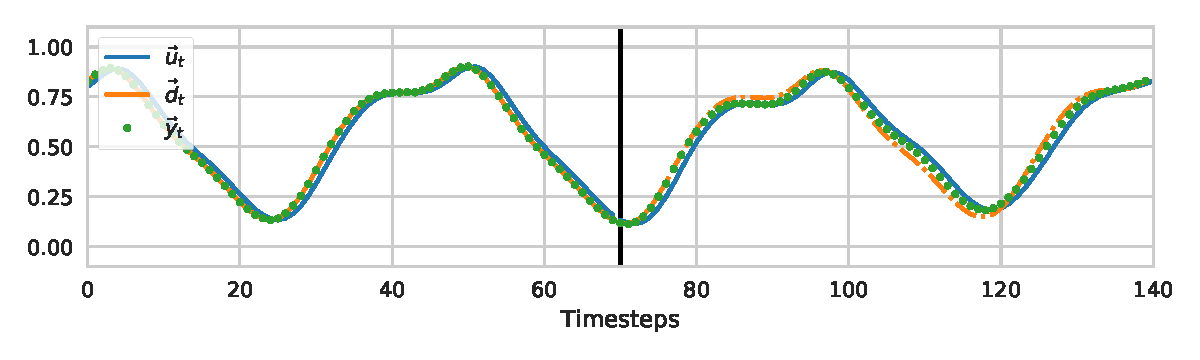
\includegraphics[width=\linewidth]{train_predict_mode.pdf}
  \caption{Input $\vt{u}$, target $\vt{d}$, and prediction $\vt{y}$ during the
  regression phase (left of the black line) and during the prediction phase.
  In the prediction phase the algorithm has no access to the true target
  any more, which is why they are depicted by a dashed line.}
  \label{fig:train_predict_mode}
\end{figure}

\subsubsection{Auto-regressive Integrated Moving Average}
\label{sub:arma}

Auto-regressive integrated moving average (ARIMA) models are widely used in
forecasting and are typically applied to non-stationary time series.  A
non-seasonal ARIMA model is defined by three parameters $p$, $q$, and $d$.  The
first parameter $p$ is the order of the auto-regressive (AR) model, $q$ is the
order of the moving-average (MA) model, and $d$ is the number of non-seasonal
differences that are needed to obtain a stationary time series.  This means
that $Y_t$ is the result of applying the sequence difference operator $\Delta
y_t = y_{t+1}-y_{t}$ for $d$ times to $y_t$:
\begin{equation}
  Y_t = \Delta^d y_t = \sum_{k=0}^d (-1)^{d-k} \binom{d}{k} y_{t+k}
\end{equation}

With the difference $Y_t$ we can write the general forcasting equation of the
ARIMA model:
\begin{equation}
  y_t = \mu + \sum_{i=1}^p \varphi_i Y_{t-i} + \sum_{i=1}^q \theta_i \epsilon_{t-i}
\end{equation}

where $\mu$ is the mean of the series, $\varphi_i$ are the $p$ parameters of
the AR model, $\theta_i$ the parameters of the MA model, and $\epsilon_i$ white
noise error terms.  The parameters of the MA and AR models have to be fit to
the data and the order of the difference must chosen a priori.


\subsubsection{Holt-Winters Method}
\label{sub:holt_winters_method}

The Holt-Winters method belongs to the class of exponential smoothing
algorithms.  In contrast to MA models that apply the same weights over a window
of a time series, exponential smoothing uses exponentially decaying weights
back in time.

The most basic form is called simple exponential smoothing (SES), where the
level of previous points provides an estimate for the next time step.  The
method maintains an estimated point $\vt{y}$, which is calculated based on
previous points and estimates.  They are assigned weights, which decrease
exponentially going back in time.
\begin{align}
  y_t = \alpha d_t + (1-\alpha)y_{t-1}
\end{align}
The smoothing parameter $\alpha$ determines exponentially
decreasing weights that are applied to previous data points.  The smoothing
parameter is chosen such that the mean squared error of prediction and data
point is minimized.

The Holt-Winters method extends the SES approach from only forecasting the level
to smoothing equations for trend $b_t$ and seasonal $s_t$.
It is described by the following four equations:
\begin{align}
  l_t &= \alpha(d_t - s_{t-L}) + (1-\alpha)(y_{t-1} + b_{t-1}) &\text{level} \\
  b_t &= \beta(l_t - l_{t-1}) + (1-\beta)b_{t-1} &\text{trend} \\
  s_t &= \gamma(y_t - l_t) + (1 - \gamma)s_{t-L} &\text{seasonal} \\
  y_{t+m} &= l_t + m b_t + s_{t-L+1+(m-1) \bmod L} &\text{forecast}
\end{align}

where $L$ is the length of the seasonal component, $\alpha$, $\beta$, $\gamma$
are constants that need to be fit to the data and $m$ denotes how far into
the future the prediction goes.


\subsection{Anomaly Score}%
\label{sub:anomaly_score}

\begin{figure}
  \centering
  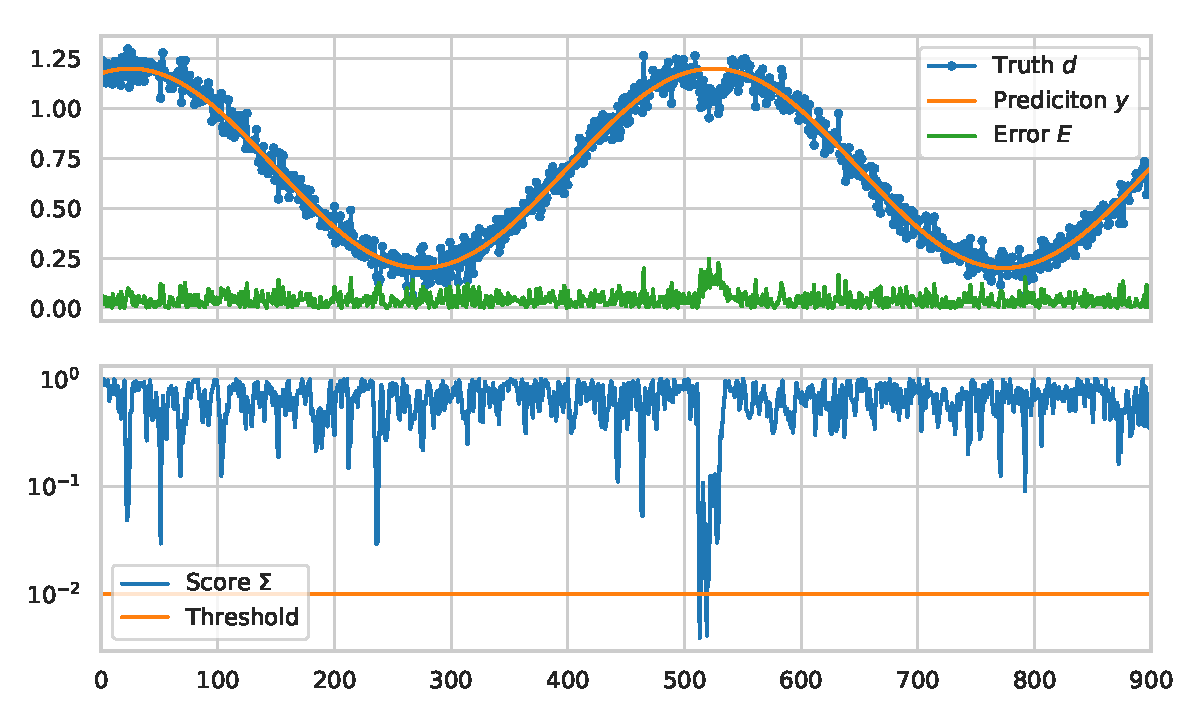
\includegraphics[width=\linewidth]{anomaly_score.pdf}
  \caption{With a good prediction $y$, the problem can be reduced to a simple
    anomaly detection over the error sequence $E$ (upper plot). The error
    sequence still takes on arbitrary values and can be converted into a
    probability of normality with an anomaly score (lower plot).
    The normality is calculated with sliding windows of length 100 for $\mu_E$
    and a length of 5 for $m_e$.
  }
  \label{fig:anomaly_score}
\end{figure}

With the predicted sequence $\textbf{y}$ it becomes quite simple to detect an
outlier, because the problem can be reduced to a \emph{simple anomaly} by
calculating the absolute error sequence $E$.

\begin{equation}
  \label{eq:err_seq}
  E_i = || \vt{y} - \vt{d} ||_2
\end{equation}

The error can now be thresholded to detect an anomaly, but the value of this
threshold depends on the specific dataset that is being analyzed.  To obtain a
probability for how anomalous a point or subsequence is, an \emph{anomaly
score} $\Sigma$ is defined as suggested by [\cite{numenta_realtime}]:

\begin{equation}
  \label{eq:normality_score}
  \Sigma = 1 - \text{erf}\bigg(\frac{\mu_e - \mu_E}{\sqrt{2}\sigma_E}\bigg),
\end{equation}

where $\mu_E$ and $\sigma_E$ denote the mean and standard deviation of a window
of length $N$ of the error sequence $E$. The mean $\mu_e$ is calculated from a
smaller subsequence of $E$ of length $n \ll N$. If $\mu_e$ is close to $\mu_E$
then $\Sigma$ will be close to one, and can thus be considered \emph{normal}
with a high probability. If $\mu_e$ and $\mu_E$ are far apart, the probability
of normality is low and the point becomes more likely to be an
outlier. This results in a score for the whole sequence, which can be used as
an intuitive threshold according to the problem at hand.
Fig.~\ref{fig:anomaly_score} shows how the anomaly detection problem of a
contextual outlier is first reduced to a simple anomaly by calculating $E$ and
then detected with a threshold on $\Sigma$. 

If the quantities $\vt{y}$ and $\vt{d}$ are vectors or matrices it might be
desirable to know which components in the vector (matrix) caused the anomaly.
For such a spatially resolved anomaly score the norm from Eq.~\ref{eq:err_seq}
can be removed and $\Sigma$ is calculated component-wise for every
coefficient in $|\vt{y} - \vt{d}|$.
